\chapter{{\em In vitro} Synthetic Biology}

In this chapter we explore biochemical networks that can be built {\em
  in vitro}, or in a test tube, out of simple molecules. We can use
short strands of DNA that interact in ways similar to how RNA
interacts inside cells, but without all of the other interactions seen
inside cells \cite{winfree-logic}. We can also add enzymes, such as
RNA polymerase, that allow us to explore transcription inside a test
tube \cite{kim-winfree-bistable}, once again without all of the other
interactions seen inside cells.

\section{Enzyme Free DNA Circuits}

\subsection{Mechanisms}

Hybridization, strand invasion, displacement, FRET.

\subsection{Design Constraints}

Sequence independence, toeholds and kinetics, secondary structure.

\subsection{Structure Prediction Software}

\subsection{The Design of an OR Gate}

\subsection{Three Different AND Gates}

In this section, we describe three different mechanisms for making an
AND gate. Each one uses the same reporter complex, which consists of
two strands as shown in Figure~\ref{fig:reporter}(a). The top strand
has the fluorophore, TAMRA, attached to it. The bottom strand has a
quencher, BHQ or Black Hole Quencher, attached to it. The reporter
does not fluoresce due to the proximity of the fluorophore and the
quencher. To use the reporter, an input strand can be introduced that
displaces the top strand. Once the top strand is displaced and moves
away from the quencher, the top strand fluoresces.

\begin{figure}
  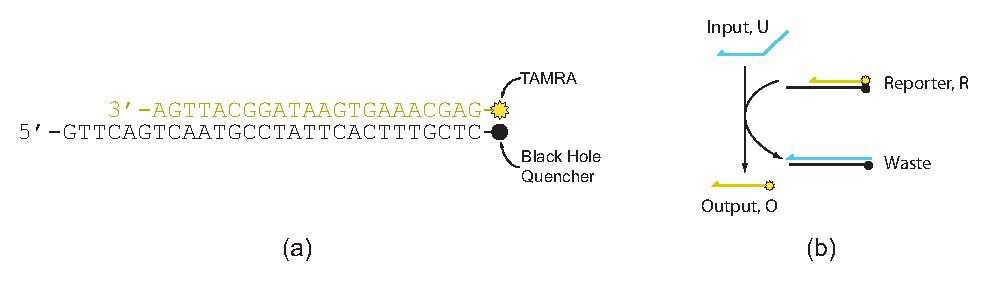
\epsfig{file=figures/invitro/reporter.eps, scale=0.8}
  \caption{\label{fig:reporter} The reporter used for the logic gate
    design problem. (a) Sequence design. (b) Use of an input strand to
    displace the fluorophore-labeled strand. }
\end{figure}

The first AND gate design, shown in Figure~\ref{fig:and1}, consists of a
backbone strand (grey) and a toehold strand (magenta) and an
intermediate strand (blue). The first input to the and gate, $A$,
attaches to the toehold and, through strand invasion, removes the
toehold strand, resulting in an intermediate complex and a waste
complex. Removing the magenta strand exposes a second toehold that is
complentary to part of input $B$, which attaches and displaces the
blue intermediate. The blue intermediate then interacts with the
reported to produce a fluorescent signal.

\begin{figure}
  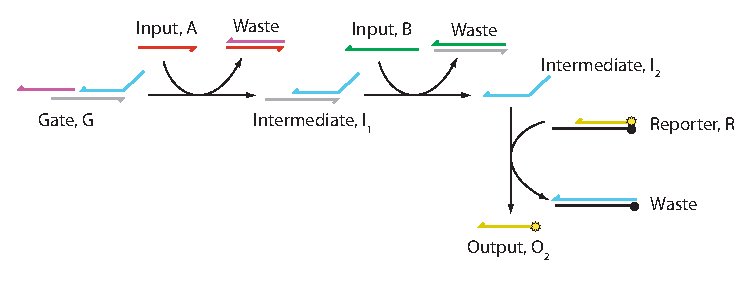
\epsfig{file=figures/invitro/and-1.eps}
  \caption{\label{fig:and1} First design for an AND gate. Input $A$ binds to the gate
    $G$, enabling input $B$ to bind.}
\end{figure}

The second AND gate design, shown in Figure~\ref{fig:and2}, is similar to the
first and gate, expect that the first input $A$ binds to the grey
backbone strand. The other main difference is that the input $A$ and
the magenta strand essentially compete as equals for the grey backbone
strand, making the first step of the process reversible. 

\begin{figure}
  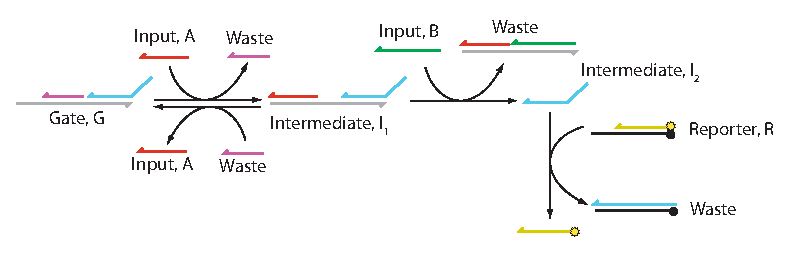
\epsfig{file=figures/invitro/and-2.eps}
  \caption{\label{fig:and2}Second design for an AND gate. Input $A$ binds to the gate
    $G$, enabling input $B$ to bind. This design differs from the
    first design in that $A$ can reversibly bind to the gate.}
\end{figure}

In both of the first two AND gate designs, input $A$ must bind to the
gate before $B$ can. The third AND gate design, shown in
Figure~\ref{fig:and3}, is symmetric in how the inputs attach to the
gate. Either can bind, and unbind first. Only once the second input
binds, the process cannot go back.

\begin{figure}
  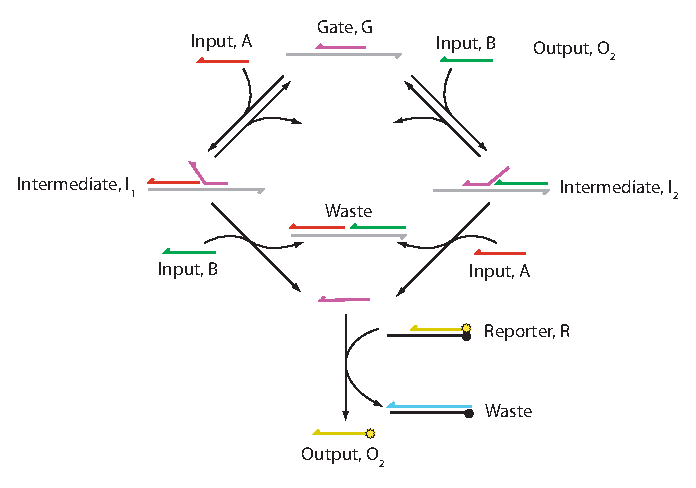
\epsfig{file=figures/invitro/and-3.eps}
  \caption{\label{fig:and3}Third design for an AND gate. Input $A$ and $B$ both
    reversibly binds to the gate $G$ to make an intermediate. The
    inputs can then bind irreversibly to complete the
    interaction. This allows the inputs to bind to the gate in either
    order.}
\end{figure}

\section{Transcriptional Circuits}

\section{Problems}

\setcounter{exercount}{0}

\begin{exercise}
  Describe each of the AND gates in
  Figure~\ref{fig:and1}-\ref{fig:and3} in terms of mass action
  kinetics and simulate them using mass action kinetics using all
  combinations of the presense or absense of the input strands. Assume the rate constants are identical
  for all bi-molecular reactions. 
\end{exercise}

\begin{exercise}
  In this problem you will design sequences to build your own DNA
  logic gate.  

  (a) Using the May 1, 2009 lecture as a guide, design sequences for
  an AND gate. Show the pairwise interactions between your strands
  predicted by NuPack, and also the results of each step in the
  reaction predicted by NuPack. You should name your sequences
  according to the scheme $GRPxSTDy$ where $x$ is your group number
  and $y$ is the strand number. Send your sequence designs to Kevin
  Oishi (koishi@u.washington.edu) by May 6 at 9:30 AM.

  (b) Simulate your AND gate using mass action kinetics using all
  combinations of the presense or absense of the input strands. Assume
  that the reaction rate for each step is proportional to the number
  of bases in the toehold region that initiate the interaction. Use
  the following table to determine which AND gate design to use:
\begin{center}
\begin{tabular}{l|l}
Group & Design \\
\hline
1 & 1 \\
2 & 2 \\
3 & 3 \\
4 & 1 \\
5 & 2 \\
6 & 3 \\
7 & 1 \\
8 & 2 \\
9 & 3 \\
10 & 1
\end{tabular}
\end{center}
\end{exercise}

\begin{exercise}
  Design a system of interacting DNA strands (using no enzymes
  whatsoever) that implements a three input AND gate. You can design
  the topology of the strands and the domains, but do not need to
  design the actual sequences (unless you want to). Show simulations
  of your system using reasonable assumptions for every combination of
  the three inputs.
\end{exercise}

\begin{exercise}
  (A Transcriptional Pulse Generator) (a) Design a transcriptional system
  (using DNA, RNA, RNAP and RNase H as in \cite{kim-winfree-bistable})
  that implements the following network: 
%
\begin{center}
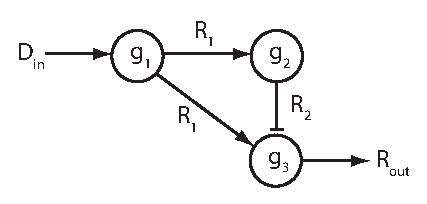
\epsfig{file=figures/trans-pulse.eps, scale=0.8}
\end{center}
%
where $g_1$, $g_2$ and $g_3$ are transcriptional swtiches, $R_1$,
$R_2$ and $R_\mathit{out}$ are RNA transcripts, and $D_\mathrm{in}$ is
a DNA input signal. For this we use a DNA input signal because we
don't want it to degrade via RNase H. Design the topology and the
domains, but not the sequences. (b) Derive equations for this system
based on regulatory network kinetics. (c) Simulate the system from an
initial condition in which all RNAs have zero concentration and
$D_\mathit{in}$ is a step input (i.e. it goes from zero to a nonzero
constant instantaneously). You should see a pulse in $R_\mathit{out}$.
\end{exercise}